\documentclass[preview]{standalone}
\usepackage{tikz}
\begin{document}
\thispagestyle{empty}
\centering
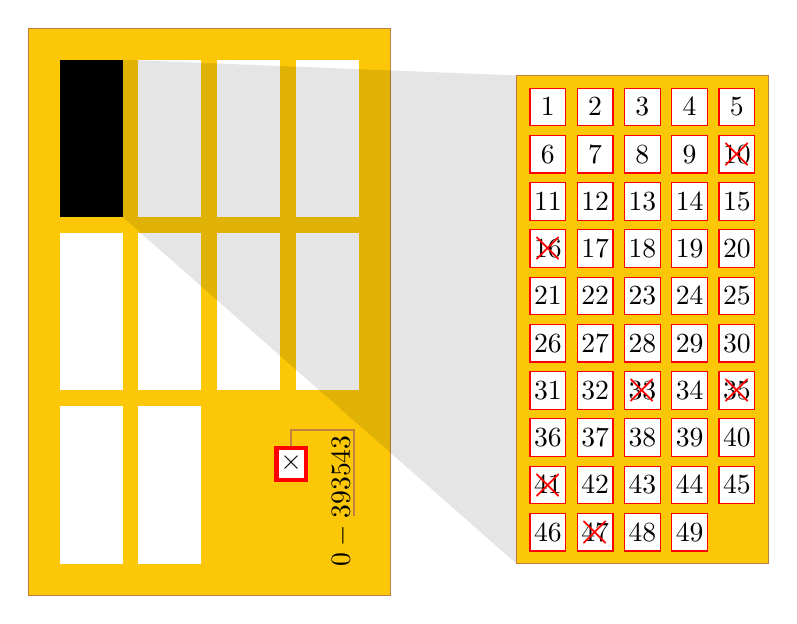
\begin{tikzpicture}[scale=2]
% ticket
\path[draw=brown, fill=yellow!60!orange] (0, 1.4) rectangle ++(2.3, 3.6);
\path[fill=black] (.2, 4.8) rectangle ++(.4, -1);
\path[fill=white] (.7, 4.8) rectangle ++(.4, -1);
\path[fill=white] (1.2, 4.8) rectangle ++(.4, -1);
\path[fill=white] (1.7, 4.8) rectangle ++(.4, -1);
\path[fill=white] (.2, 3.7) rectangle ++(.4, -1);
\path[fill=white] (.7, 3.7) rectangle ++(.4, -1);
\path[fill=white] (1.2, 3.7) rectangle ++(.4, -1);
\path[fill=white] (1.7, 3.7) rectangle ++(.4, -1);
\path[fill=white] (.2, 2.6) rectangle ++(.4, -1);
\path[fill=white] (.7, 2.6) rectangle ++(.4, -1);
\path (2, 2) node [rotate=90] {$0-393543$\strut};
\path[draw=brown, thick] (2.07, 1.9) |- ++(-.4, .55) -- ++(0, -.1)
	node [below, draw=red, ultra thick, fill=white, inner sep=0, minimum width=2.5ex, text height=.8em] {$\times$\strut};
%
\path (3.1, 1.6) node (col) {};
\path[draw=brown, fill=yellow!60!orange] (col) rectangle ++(1.6, 3.1);
\path (col)++(.2, 2.9) node [fill=white, draw=red, inner sep=0, minimum width=3ex, text height=1em] {$1$\strut};
\path (col)++(.5, 2.9) node [fill=white, draw=red, inner sep=0, minimum width=3ex, text height=1em] {$2$\strut};
\path (col)++(.8, 2.9) node [fill=white, draw=red, inner sep=0, minimum width=3ex, text height=1em] {$3$\strut};
\path (col)++(1.1, 2.9) node [fill=white, draw=red, inner sep=0, minimum width=3ex, text height=1em] {$4$\strut};
\path (col)++(1.4, 2.9) node [fill=white, draw=red, inner sep=0, minimum width=3ex, text height=1em] {$5$\strut};
\path (col)++(.2, 2.6) node [fill=white, draw=red, inner sep=0, minimum width=3ex, text height=1em] {$6$\strut};
\path (col)++(.5, 2.6) node [fill=white, draw=red, inner sep=0, minimum width=3ex, text height=1em] {$7$\strut};
\path (col)++(.8, 2.6) node [fill=white, draw=red, inner sep=0, minimum width=3ex, text height=1em] {$8$\strut};
\path (col)++(1.1, 2.6) node [fill=white, draw=red, inner sep=0, minimum width=3ex, text height=1em] {$9$\strut};
\path (col)++(1.4, 2.6) node [fill=white, draw=red, inner sep=0, minimum width=3ex, text height=1em] {$10$\strut}
	node[red] {\LARGE$\times$\strut};
\path (col)++(.2, 2.3) node [fill=white, draw=red, inner sep=0, minimum width=3ex, text height=1em] {$11$\strut};
\path (col)++(.5, 2.3) node [fill=white, draw=red, inner sep=0, minimum width=3ex, text height=1em] {$12$\strut};
\path (col)++(.8, 2.3) node [fill=white, draw=red, inner sep=0, minimum width=3ex, text height=1em] {$13$\strut};
\path (col)++(1.1, 2.3) node [fill=white, draw=red, inner sep=0, minimum width=3ex, text height=1em] {$14$\strut};
\path (col)++(1.4, 2.3) node [fill=white, draw=red, inner sep=0, minimum width=3ex, text height=1em] {$15$\strut};
\path (col)++(.2, 2.0) node [fill=white, draw=red, inner sep=0, minimum width=3ex, text height=1em] {$16$\strut}
	node[red] {\LARGE$\times$\strut};
\path (col)++(.5, 2.0) node [fill=white, draw=red, inner sep=0, minimum width=3ex, text height=1em] {$17$\strut};
\path (col)++(.8, 2.0) node [fill=white, draw=red, inner sep=0, minimum width=3ex, text height=1em] {$18$\strut};
\path (col)++(1.1, 2.0) node [fill=white, draw=red, inner sep=0, minimum width=3ex, text height=1em] {$19$\strut};
\path (col)++(1.4, 2.0) node [fill=white, draw=red, inner sep=0, minimum width=3ex, text height=1em] {$20$\strut};
\path (col)++(.2, 1.7) node [fill=white, draw=red, inner sep=0, minimum width=3ex, text height=1em] {$21$\strut};
\path (col)++(.5, 1.7) node [fill=white, draw=red, inner sep=0, minimum width=3ex, text height=1em] {$22$\strut};
\path (col)++(.8, 1.7) node [fill=white, draw=red, inner sep=0, minimum width=3ex, text height=1em] {$23$\strut};
\path (col)++(1.1, 1.7) node [fill=white, draw=red, inner sep=0, minimum width=3ex, text height=1em] {$24$\strut};
\path (col)++(1.4, 1.7) node [fill=white, draw=red, inner sep=0, minimum width=3ex, text height=1em] {$25$\strut};
\path (col)++(.2, 1.4) node [fill=white, draw=red, inner sep=0, minimum width=3ex, text height=1em] {$26$\strut};
\path (col)++(.5, 1.4) node [fill=white, draw=red, inner sep=0, minimum width=3ex, text height=1em] {$27$\strut};
\path (col)++(.8, 1.4) node [fill=white, draw=red, inner sep=0, minimum width=3ex, text height=1em] {$28$\strut};
\path (col)++(1.1, 1.4) node [fill=white, draw=red, inner sep=0, minimum width=3ex, text height=1em] {$29$\strut};
\path (col)++(1.4, 1.4) node [fill=white, draw=red, inner sep=0, minimum width=3ex, text height=1em] {$30$\strut};
\path (col)++(.2, 1.1) node [fill=white, draw=red, inner sep=0, minimum width=3ex, text height=1em] {$31$\strut};
\path (col)++(.5, 1.1) node [fill=white, draw=red, inner sep=0, minimum width=3ex, text height=1em] {$32$\strut};
\path (col)++(.8, 1.1) node [fill=white, draw=red, inner sep=0, minimum width=3ex, text height=1em] {$33$\strut}
	node[red] {\LARGE$\times$\strut};
\path (col)++(1.1, 1.1) node [fill=white, draw=red, inner sep=0, minimum width=3ex, text height=1em] {$34$\strut};
\path (col)++(1.4, 1.1) node [fill=white, draw=red, inner sep=0, minimum width=3ex, text height=1em] {$35$\strut}
	node[red] {\LARGE$\times$\strut};
\path (col)++(.2, .8) node [fill=white, draw=red, inner sep=0, minimum width=3ex, text height=1em] {$36$\strut};
\path (col)++(.5, .8) node [fill=white, draw=red, inner sep=0, minimum width=3ex, text height=1em] {$37$\strut};
\path (col)++(.8, .8) node [fill=white, draw=red, inner sep=0, minimum width=3ex, text height=1em] {$38$\strut};
\path (col)++(1.1, .8) node [fill=white, draw=red, inner sep=0, minimum width=3ex, text height=1em] {$39$\strut};
\path (col)++(1.4, .8) node [fill=white, draw=red, inner sep=0, minimum width=3ex, text height=1em] {$40$\strut};
\path (col)++(.2, .5) node [fill=white, draw=red, inner sep=0, minimum width=3ex, text height=1em] {$41$\strut}
	node[red] {\LARGE$\times$\strut};
\path (col)++(.5, .5) node [fill=white, draw=red, inner sep=0, minimum width=3ex, text height=1em] {$42$\strut};
\path (col)++(.8, .5) node [fill=white, draw=red, inner sep=0, minimum width=3ex, text height=1em] {$43$\strut};
\path (col)++(1.1, .5) node [fill=white, draw=red, inner sep=0, minimum width=3ex, text height=1em] {$44$\strut};
\path (col)++(1.4, .5) node [fill=white, draw=red, inner sep=0, minimum width=3ex, text height=1em] {$45$\strut};
\path (col)++(.2, .2) node [fill=white, draw=red, inner sep=0, minimum width=3ex, text height=1em] {$46$\strut};
\path (col)++(.5, .2) node [fill=white, draw=red, inner sep=0, minimum width=3ex, text height=1em] {$47$\strut}
	node[red] {\LARGE$\times$\strut};
\path (col)++(.8, .2) node [fill=white, draw=red, inner sep=0, minimum width=3ex, text height=1em] {$48$\strut};
\path (col)++(1.1, .2) node [fill=white, draw=red, inner sep=0, minimum width=3ex, text height=1em] {$49$\strut};
%
\path [fill=black, very nearly transparent] (.6, 4.8) -- (.6, 3.8) -- (col.center) -- ++(0, 3.1) -- cycle;

\end{tikzpicture}
\end{document}